\chapter{Methodology}
In this chapter we present a detailed problem analysis and discuss our approach for solving the issue.
\label{mainone}
% DELETEME: In this chapter you start addressing your actual problem. Therefore, it makes often sense to make a detailed problem analysis first (if not done in introduction). You should be sure about what to do and how. While writing in the background part, it might also make sense to include complex background information or papers you are basing on in this analysis. If you are solving a software problem, you should follow the state of the art of software development which basically includes: problem analysis, design, implementation, testing, and deployment. Maintenance is often also described but I believe this will not be required for most theses. Code should be placed in the appendix unless it is solving an essential aspect of your work.
\section{Problem Anlaysis}



\section{Approach for Solving the Issue}
This section provides an explanation of what techniques were used in the problem's solution. It is split into smaller subsections, which consider different parts of the proposed strategy.

\subsection{Organisation of the Simulation}
In general, to conduct real-world experiments is rather expensive and time-consuming, therefore we simulate different scenarios using CARLA. What is more, there are no limitations in the digital environment and data samples can be created faster, which contain no distortions or noise. It offers an opportunity to test different approaches and ideas in ideal conditions without any restrictions.

Our simulation takes place in a realistic digital city "Town10HD\_Opt" from the CARLA assets package, which represents a whole town including, i.e., buildings, trees, traffic lights, parked vehicles, etc. The main location of the experiments is a junction of four roads, because, compared to other types of intersections, there exists a higher chance for accidents to happen, and an optimal camera placement is crucial for a safe mobility. On the junction's premises we place 3 CARLA objects from type Actor: 
\begin{itemize}
    \item 1 camera and 2 vehicles, which has the roles 'occluder' and 'target'
\end{itemize}
In pursuance of finding an optimal position for the camera sensor we consider the 4 angles of the region of interest (ROI) and also the points in the middle of each of the 4 edges like it is shown in Figure \ref{fig:camera_positions}. In this way, we earn an approximate idea which point or area has to be aimed for when placing a camera. Furthermore, this placement could be applied to other infrastructure of the same type, therefore it also guarantees flexibility and universality of the approach. 

With regard to the vehicles, which play the most important role in our research, we divide them into two categories:

\begin{itemize}
    \item \textbf{occluder vehicle} - this is the vehicle that stays between the sensor and the target vehicle and covers some part of it because of its larger size or position regarding the sensor. For a realistic scenario we use a medium and large-sized vans or trucks, so that their shape generate a blind zone for the sensor's field of view, which then cannot recognize the occluded vehicle. 
    \item \textbf{target vehicle} - this vehicle is equal or smaller than the occluder, because we have to measure the degree to which it is occluded in various positions. If, for example, it has the bigger proportions, the chance of a camera not detecting it is quite decreased even if it stays behind the occluder. 
\end{itemize}
During the simulation we spawn both vehicles in different locations on the intersection in order to reproduce as many as possible dynamic situations and decide whether an occlusion occurs or not.

\begin{figure} [h]
    \centering
    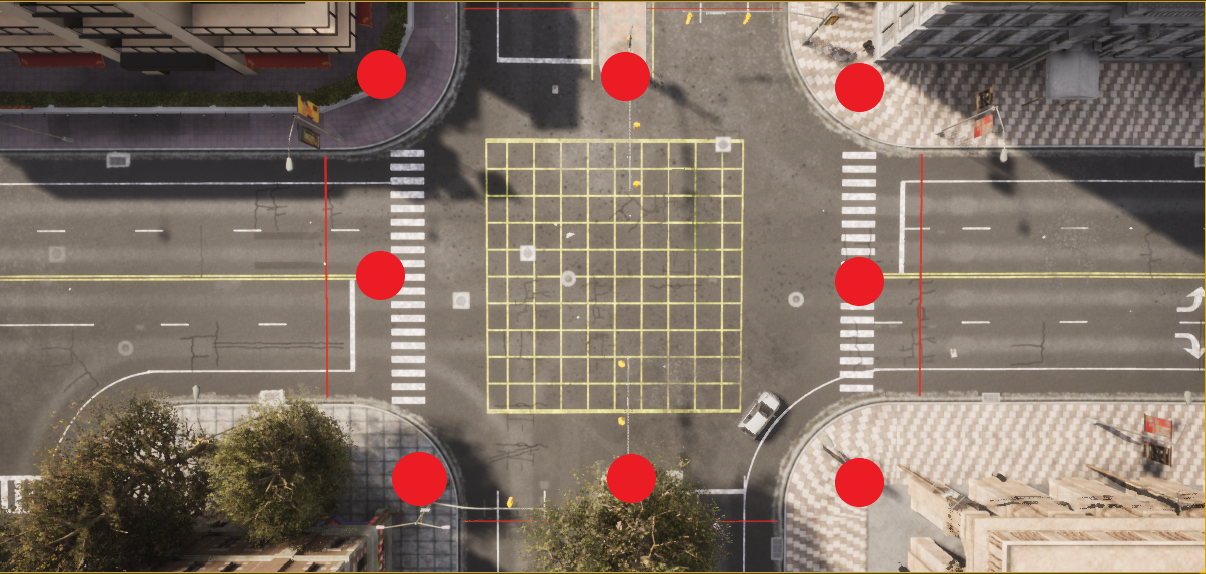
\includegraphics[width=\textwidth]{images/junction.png}
    \caption[Camera experiment positions]{This picture displays an example where the camera is going to be placed during simulations}
    \label{fig:camera_positions}
\end{figure}

\subsection{Simulation Pipeline}

This thesis relies on a simulation pipeline for conducting experiments and evaluating their output, which consists of three main stages that can be seen on Figure \ref{fig:evaluation_pipeline}: 

\begin{enumerate}
    \item \textbf{Preparation of the experiment} - encompasses the configuration of all virtual world settings, as well as the creation of points on the test intersection that will be used during the experiments. In this stage a camera object is spawned within the simulated environment, which perceives the traffic and returns data that has to be evaluated. 
    \item \textbf{Reproduction of possible scenarios} - during this stage we have tuples of vehicles(occluder and target) that are spawned on the waypoints generated in the previous stage. In addition, after each new spawn, images from the camera are saved for further evaluation of the occlusion degree and the other metrics.
    \item \textbf{Evaluation of results} - being the last stage of the simulation pipeline, here the results are evaluated and used to generate a heatmap and a graph for a better visualisation, after which we discuss in \ref{evaluation} how our approach optimises traffic camera placement.
\end{enumerate}
In the following subsections we provide a more detailed explanation of how all the process from data generation via vehicles placement to output evaluation is realised.
\begin{figure} [h]
    \centering
    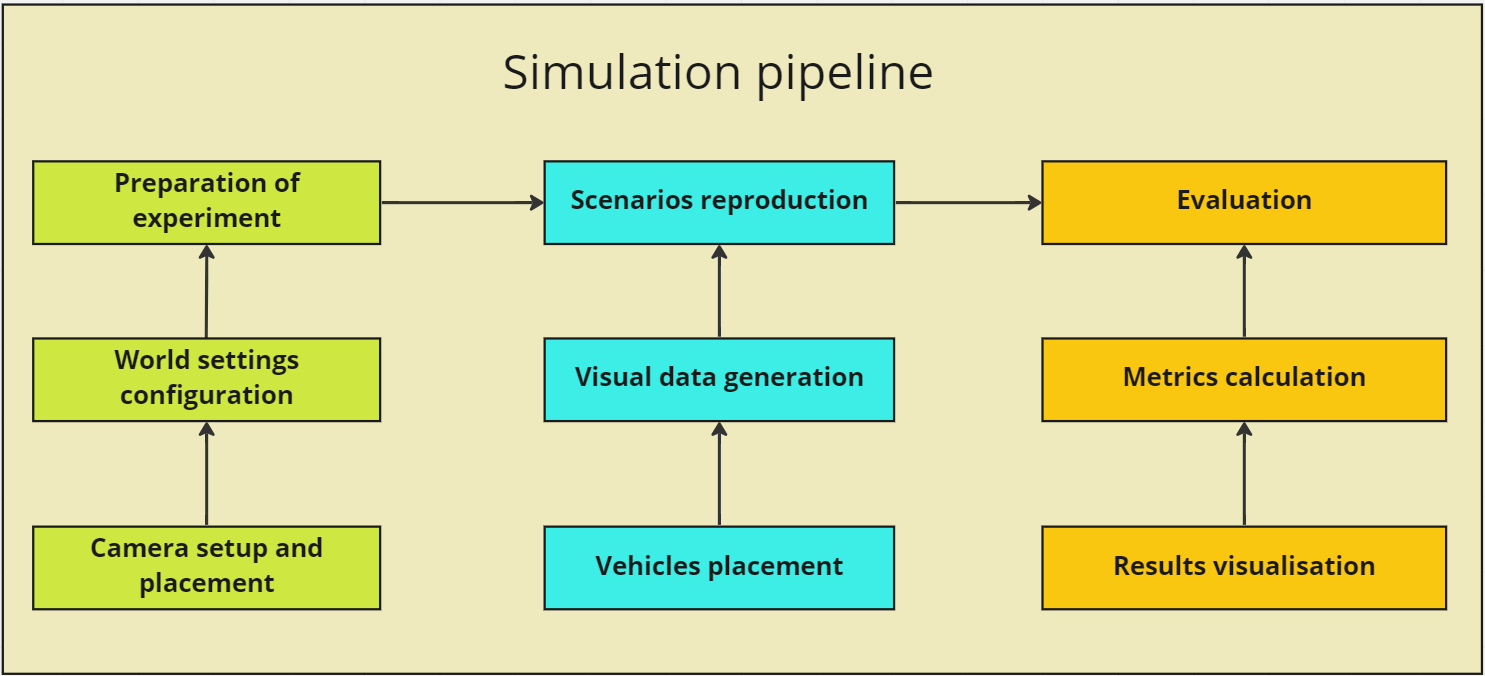
\includegraphics[width=\textwidth]{images/evaluation_pipeline.png}
    \caption[Evaluation pipeline]{This diagram represents schematically the simulation pipeline}
    \label{fig:evaluation_pipeline}
\end{figure}

\subsection{Experiment Setup and Environment Preparation}
Before each simulation it is important to adjust the world settings correctly in order to maintain a synchronous mode, which allows for reliable data from the sensors. In CARLA we set a client which communicates with our world and a traffic manager which is responsible for the behaviour of vehicles. 

When we are done with the creation of our simulated environment, the main priority is to generate waypoints within the intersection, which serve as spawn points for the vehicle actors.